\clearpage
\section{Validierung und Verifizierung}\label{sec:ValidierungVerifizierung}

\subsection{Validierung}\label{subsec:Validierung}
Die durchgeführten Messungen haben aussagekräftige Resultate geliefert welche jedoch stark vom gewählten Vorgehen abhängig sind. Dieses Vorgehen soll nun kritisch überprüft und allfällige Mängel im Konzept sowie der Umsetzung aufgezeigt werden. Zudem werden systematische Messfehler deklariert.

\paragraph{Large Payload}
Die Resultate der Messreihen 3, 4 und 8, welche mit einer grossen Payload durchgeführt wurden, sind nur für Thread und Zigbee aussagekräftig. Der BT Mesh Stack liefert bei diesen Messungen keine brauchbaren Resultate. Eine Recherche zu diesem Problem hat ergeben, dass durch die Fragmentierung einer 32 Byte Payload die sichere und schnelle Übertragung der Daten nicht mehr gewährleistet werden kann.

\paragraph{Zigbee Latency}
Wie bereits erwähnt, konnte bei Zigbee die Anzahl Hops die ein Paket passiert hat nicht ausgewertet werden.
Der Forumsbeitrag \href{https://devzone.nordicsemi.com/f/nordic-q-a/63815/zigbee---read-number-of-hops-radius}{\textit{Zigbee - Read number of hops (radius)\footnote{\url{https://devzone.nordicsemi.com/f/nordic-q-a/63815/zigbee---read-number-of-hops-radius}}}} bestätigt, dass der entsprechende Wert mit der verwendeten SDK nicht ausgelesen werden kann.
Als Folge dessen kann schliesslich die Latenzzeit nur als Total über die gesamte Strecke erfasst werden. In der Auswertung verschafft dies BT Mesh und Thread fälschlicherweise einen Vorteil gegenüber Zigbee.
Die Auswertung der totalen Latenzzeit bei allen 3 Protokollen könnte das Problem lösen.
Dies würde jedoch dem Messkonzept widersprechen und wurde deshalb nicht für alle Messungen umgesetzt.
Die Abbildungen \ref{fig:DurchschnittlicheLatenzzeitValidierung} und \ref{fig:DurchschnittlicheLatenzzeitohneHopsValidierung} zeigen den Unterschied am Beispiel der oben analysierten Messung \ref{sec:Ergebnisse}.
Während links die Latenzzeit pro Hop dargestellt ist, zeigt die rechte Grafik die totale Latenzzeit.
Der Unterschied ist vorallem bei Thread deutlich erkennbar.
Bereits in der Abbildung \ref{fig:VerteilungderLatenzzeiten} ist das Problem zu erkennen.
Die Statistik der Latenzzeiten von Zigbee hat zwei Hauptsäulen bei 40ms und 70ms was auf einen Hop hindeutet.


\begin{figure}[!htbp]
	\centering
	\begin{minipage}[b]{0.49\textwidth}
		\centering
		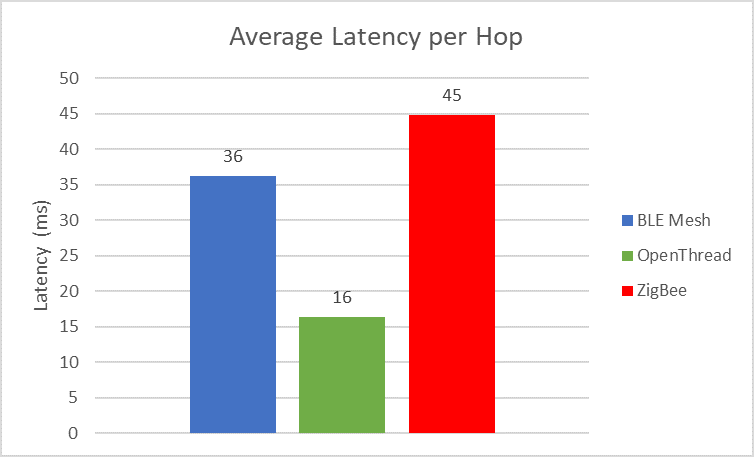
\includegraphics[width=\textwidth]{Average_Latency_per_Hop.png}
		\caption{Durchschnittliche Latenzzeit pro Hop}
		\label{fig:DurchschnittlicheLatenzzeitValidierung}
	\end{minipage}
	\begin{minipage}[b]{0.49\textwidth}
		\centering
		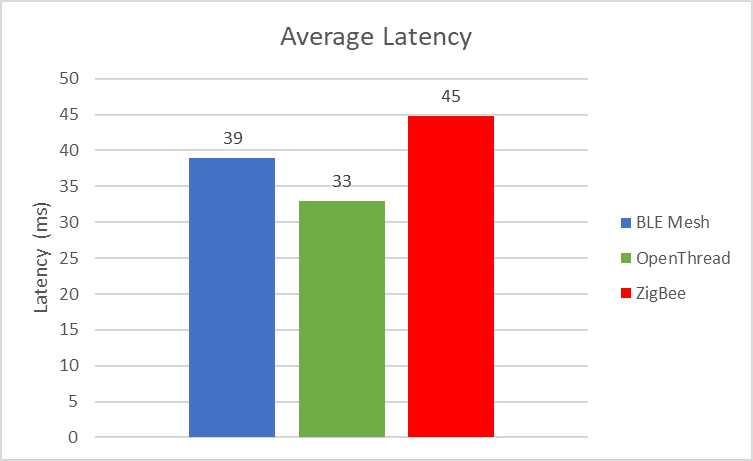
\includegraphics[width=\textwidth]{Average_Latency_without_Hops.png}
		\caption{Durchschnittliche Latenzzeit ohne Berücksichtigung der Hops.}	\label{fig:DurchschnittlicheLatenzzeitohneHopsValidierung}
	\end{minipage}
\end{figure}

\newpage
\paragraph{Nachrichten Dichte}
Bei der Definition der Messreihen \ref{sec:Interpretation} wurden zu Beginn nur die Messungen 1 bis 6 spezifiziert.
Die Messreihen 7 und 8 kamen erst nachträglich hinzu als festgestellt werden musste, dass die Dichte der Nachrichten für den BT Mesh Stack zu hoch gewählt wurde.
Dieser schien überfordert besonders bei zufälliger Nachrichten Generierung.
Thread und Zigbee zeigten indes keine Mühe mit der Dichte von 60 Nachrichten in 600 Sekunden pro Node.
Die Resultate der Messungen 7 und 8 haben schliesslich gezeigt, dass die Reduktion der Nachrichtendichte einen positiven Einfluss hat.

\paragraph{Group addressing mode}
Der \textit{Group addressing mode} wurde für die 3 Protokolle unterschiedlich definiert.
Erste Tests vor den eigentlichen Benchmarks haben gezeigt, dass eine Multicast Adressierung bei Zigbee unbrauchbar ist.
Deshalb hat man sich entschieden bei Zigbee eine Unicast Adressierung umzusetzen.
Während den Benchmarks musste schliesslich festgestellt werden, dass Zigbee durch diese Änderung ein deutlicher Vorteil erlangt hat.
Besonders auf die Paketverlustrate hat sich die Unicast Adressierung positiv ausgewirkt denn Unicast Nachrichten werden im IEEE 802.15.4 Standard auf MAC Ebene quittiert.
Multicast resp. Broadcast hingegen nicht.

Auch in der Messung Nr. 5 hätte sich die Unicast Adressierung für Zigbee positiv ausgewirkt da die Netzbelastung deutlich geringer gewesen wäre.

\paragraph{Durchschnittswerte in den Resultaten}
In den Ergebnissen \ref{sec:Ergebnisse} wurden sämtliche Durchschnittswerte als Mittelwerte einschliesslich allfälliger Ausreisser aus den Messwerten gebildet.
Dadurch wurden gewisse Resultate deutlich verfälscht.
In einer neuen Auswertung müsste die Ursache für die einzelnen Ausreisser genauer geklärt werden und diese allenfalls gestrichen werden.


\subsection{Verifizierung}\label{subsec:Verifizierung}
Eine Verifizierung der Messresultate konnte nur anhand des Referenzberichts \textit{AN1142: Mesh Network Performance
	Comparison\footnote{\url{https://www.silabs.com/documents/public/application\%2Dnotes/an1142\%2Dmesh\%2Dnetwork\%2Dperformance\%2Dcomparison.pdf} \cite{silicon_laboratories_inc_an1142_2020}}} von \textit{Silicon Labs} gemacht werden.
Dieser ist auf der Webseite von \textit{Silicon Labs} einsehbar.

Der Vergleich der Messergebnisse hat gezeigt, dass die Grössenordnung der Resultate mit jenen aus dem Bericht von Silicon Labs übereinstimmt.
Selbst die Ausreisser in der Latenzzeit bei BT Mesh liegen im selben Rahmen.
Zudem kann die klare Abhängigkeit der Resultate von der Grösse der Payload bestätigt werden.
Einige Unterschiede sind jedoch in der Verteilung der Latenzzeiten erkennbar.
Im Referenzbericht ist diese in einem Bereich zwischen 20ms und 60ms ziemlich regelmässig während in den Ergebnissen dieser Thesis die Verteilung unregelmässiger daherkommt.